\documentclass[12pt,a4paper]{article}

% ── Kodowanie i język ─────────────────────────────────────────────────────
\usepackage[utf8]{inputenc}
\usepackage[T1]{fontenc}
\usepackage[polish]{babel}

% ── Czcionki i typografia ────────────────────────────────────────────────
\usepackage{lmodern}
\usepackage{microtype}

% ── Układ strony ─────────────────────────────────────────────────────────
\usepackage[margin=2.5cm]{geometry}
\usepackage{setspace}
\onehalfspacing

% ── Matematyka ───────────────────────────────────────────────────────────
\usepackage{amsmath,amssymb,amsthm}

% ── Grafika i tabele ─────────────────────────────────────────────────────
\usepackage{graphicx}
\usepackage{float}
\usepackage{booktabs}
\usepackage{caption}
\usepackage{subcaption}

% ── Hiperłącza ───────────────────────────────────────────────────────────
\usepackage[colorlinks=true,linkcolor=blue!60!black,citecolor=green!50!black,urlcolor=blue!70!black]{hyperref}

% ── Listingi kodu ────────────────────────────────────────────────────────
\usepackage{listings}
\lstset{
  language=Python,
  basicstyle=\ttfamily\small,
  keywordstyle=\bfseries\color{blue!70!black},
  commentstyle=\itshape\color{gray},
  breaklines=true,
  frame=single,
  numbers=left,
  numberstyle=\tiny\color{gray},
}

% ── Ścieżka do wykresów ──────────────────────────────────────────────────
\graphicspath{{../output/}}

% ── Metadane ─────────────────────────────────────────────────────────────
\title{%
  \textbf{Wycena i symulacja zabezpieczenia (Delta-Hedging)\\
  opcji na obligacje w~modelu Hull-White~1F}\\[0.5em]
  \large Analiza lat 2020--2024 w~środowisku gwałtownych zmian\\
  stóp procentowych
}
\author{Maksymilian Dębowski}
\date{\today}

% ══════════════════════════════════════════════════════════════════════════
\begin{document}
\maketitle
\thispagestyle{empty}

\begin{abstract}
Niniejszy raport przedstawia implementację jednoczynnikowego modelu
Hulla-White'a~(HW~1F) oraz jego zastosowanie do wyceny europejskiej opcji
kupna na obligację zerokuponową (ZCB). Model został skalibrowany do
historycznych danych krzywej dochodowości US~Treasury z~okresu 2020--2024,
obejmującego pandemię COVID-19 oraz bezprecedensowy cykl podwyżek stóp
procentowych przez Fed. Przeprowadzono symulację Monte~Carlo w~celu
weryfikacji cen analitycznych, a~następnie wykonano backtest strategii
delta-hedgingu -- zarówno na ścieżkach symulowanych, jak i~na danych
historycznych. Wyniki porównano z~modelem Vasicka, wykazując przewagę HW~1F
w~odtwarzaniu krzywej dochodowości (RMSE~$= 0{,}0$~bps vs.~$131{,}6$~bps
dla Vasicka).
\end{abstract}

\tableofcontents
\newpage

% ══════════════════════════════════════════════════════════════════════════
\section{Wprowadzenie}
\label{sec:intro}

Modelowanie stóp procentowych stanowi fundament wyceny instrumentów dłużnych
i~zarządzania ryzykiem portfeli obligacyjnych. Okres 2020--2024 dostarcza
unikalnego laboratorium do testowania modeli stochastycznych:

\begin{itemize}
  \item \textbf{2020} -- pandemia COVID-19, stopy bliskie zeru, masowy skup
        aktywów (QE);
  \item \textbf{2021} -- ożywienie gospodarcze, narastająca inflacja;
  \item \textbf{2022--2023} -- najszybszy cykl podwyżek stóp Fed od lat~80.
        (z~0\% do~5,5\%);
  \item \textbf{2024} -- stabilizacja na podwyższonym poziomie, oczekiwania
        na obniżki.
\end{itemize}

Celem projektu jest zbadanie, jak dobrze model Hull-White~1F radzi sobie
w~tym środowisku -- zarówno pod względem wyceny opcji, jak i~skuteczności
strategii zabezpieczającej (delta-hedging).

% ══════════════════════════════════════════════════════════════════════════
\section{Podstawy teoretyczne}
\label{sec:theory}

\subsection{Model Hull-White 1F}

Jednoczynnikowy model Hulla-White'a opisuje dynamikę chwilowej stopy
procentowej $r(t)$ za pomocą stochastycznego równania różniczkowego (SDE):

\begin{equation}
  \label{eq:hw-sde}
  dr(t) = \bigl[\theta(t) - a\,r(t)\bigr]\,dt + \sigma\,dW(t),
\end{equation}

gdzie:
\begin{itemize}
  \item $a > 0$ -- szybkość powrotu do średniej (\emph{mean-reversion speed}),
  \item $\sigma > 0$ -- zmienność krótkiej stopy,
  \item $\theta(t)$ -- deterministyczna funkcja czasu zapewniająca
        dokładne dopasowanie do~początkowej krzywej dochodowości,
  \item $W(t)$ -- standardowy proces Wienera.
\end{itemize}

Funkcja $\theta(t)$ wyznaczana jest z~rynkowej chwilowej stopy forward
$f^M(0,t)$:

\begin{equation}
  \label{eq:theta}
  \theta(t) = \frac{\partial f^M(0,t)}{\partial t}
              + a\,f^M(0,t)
              + \frac{\sigma^2}{2a}\bigl(1 - e^{-2at}\bigr).
\end{equation}

\subsection{Wycena obligacji zerokuponowej}

Cena ZCB w~modelu HW~1F ma postać afiniczną:

\begin{equation}
  \label{eq:zcb}
  P(t,T) = A(t,T)\,\exp\bigl(-B(t,T)\,r(t)\bigr),
\end{equation}

gdzie:
\begin{align}
  B(t,T) &= \frac{1 - e^{-a(T-t)}}{a}, \label{eq:B}\\[6pt]
  \ln A(t,T) &= \ln\frac{P^M(0,T)}{P^M(0,t)}
               + B(t,T)\,f^M(0,t)
               - \frac{\sigma^2}{4a}\,B(t,T)^2\,
                 \bigl(1 - e^{-2at}\bigr). \label{eq:lnA}
\end{align}

\subsection{Europejska opcja na ZCB -- formuła Jamshidiana}

Cena europejskiej opcji kupna (call) z~czasem wygaśnięcia $T$ na~ZCB
o~zapadalności $S > T$ i~cenie wykonania $K$:

\begin{equation}
  \label{eq:call}
  C(0) = P^M(0,S)\,\Phi(h) - K\,P^M(0,T)\,\Phi(h - \sigma_P),
\end{equation}

gdzie $\Phi(\cdot)$ oznacza dystrybuantę rozkładu normalnego, a:

\begin{align}
  \sigma_P &= \frac{\sigma}{a}\bigl(1 - e^{-a(S-T)}\bigr)
              \sqrt{\frac{1 - e^{-2aT}}{2a}}, \label{eq:sigma_p}\\[6pt]
  h &= \frac{1}{\sigma_P}\ln\frac{P^M(0,S)}{K\,P^M(0,T)}
       + \frac{\sigma_P}{2}. \label{eq:h}
\end{align}

\subsection{Delta opcji}

Wrażliwość ceny opcji na cenę obligacji bazowej (delta do~hedgingu):

\begin{equation}
  \label{eq:delta}
  \Delta = \frac{\partial C}{\partial P(t,S)} = \Phi(h).
\end{equation}

\subsection{Model Vasicka -- benchmark}

Model Vasicka stanowi szczególny przypadek, w~którym $\theta(t) = a\cdot b$
jest stałe:

\begin{equation}
  dr(t) = a\bigl(b - r(t)\bigr)\,dt + \sigma\,dW(t).
\end{equation}

Kluczowa różnica: Vasicek \textbf{nie} odtwarza dokładnie krzywej rynkowej,
co prowadzi do systematycznego błędu wyceny.

% ══════════════════════════════════════════════════════════════════════════
\section{Dane}
\label{sec:data}

\subsection{Źródło danych}

Wykorzystano dane z~\textbf{FRED} (Federal Reserve Economic Data) --
dzienne stopy US~Treasury Constant Maturity dla~11 tenorów
(Tabela~\ref{tab:series}).

\begin{table}[H]
  \centering
  \caption{Serie FRED użyte do konstrukcji krzywej dochodowości.}
  \label{tab:series}
  \begin{tabular}{@{}lll@{}}
    \toprule
    \textbf{Symbol FRED} & \textbf{Tenor} & \textbf{Zapadalność [lata]} \\
    \midrule
    DGS1MO  & 1M   & 0,083  \\
    DGS3MO  & 3M   & 0,250  \\
    DGS6MO  & 6M   & 0,500  \\
    DGS1    & 1Y   & 1,000  \\
    DGS2    & 2Y   & 2,000  \\
    DGS3    & 3Y   & 3,000  \\
    DGS5    & 5Y   & 5,000  \\
    DGS7    & 7Y   & 7,000  \\
    DGS10   & 10Y  & 10,000 \\
    DGS20   & 20Y  & 20,000 \\
    DGS30   & 30Y  & 30,000 \\
    \bottomrule
  \end{tabular}
\end{table}

Okres analizy: \textbf{2 stycznia 2020 -- 31 grudnia 2024}
(1304~obserwacji po~usunięciu braków).

\subsection{Krzywa dochodowości}

Stopy par-yield z~FRED traktowano jako ciągle składane zero-rates
i~interpolowano splajnem kubicznym, uzyskując ciągłe funkcje:
$P^M(0,T)$, $f^M(0,T)$ oraz $\partial f^M/\partial T$.

\subsection{Proxy krótkiej stopy}

Jako przybliżenie chwilowej stopy $r(t)$ przyjęto stopę 3-miesięczną
Treasury (DGS3MO). Rysunek~\ref{fig:short-rate} przedstawia jej ewolucję.

\begin{figure}[H]
  \centering
  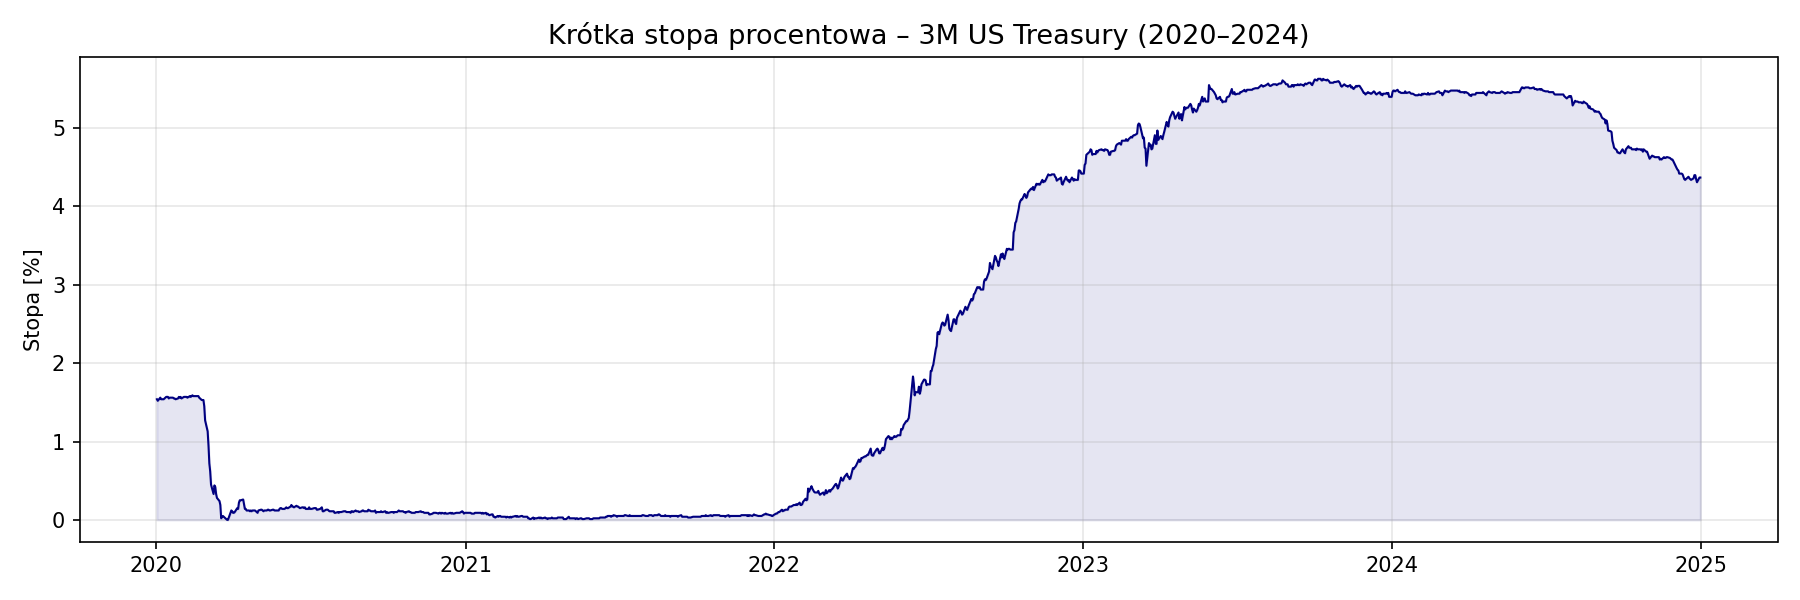
\includegraphics[width=\textwidth]{short_rate_history.png}
  \caption{Krótka stopa procentowa (3M US Treasury) w~latach 2020--2024.
           Widoczny gwałtowny wzrost z~poziomu bliskiego~0\% do ponad~5\%
           w~wyniku cyklu podwyżek Fed.}
  \label{fig:short-rate}
\end{figure}

\subsection{Ewolucja krzywej dochodowości}

Rysunek~\ref{fig:yield-3d} przedstawia trójwymiarową ewolucję całej
krzywej dochodowości, ukazując przejście od~środowiska ultra-niskich stóp
do~inwersji krzywej i~następnie normalizacji.

\begin{figure}[H]
  \centering
  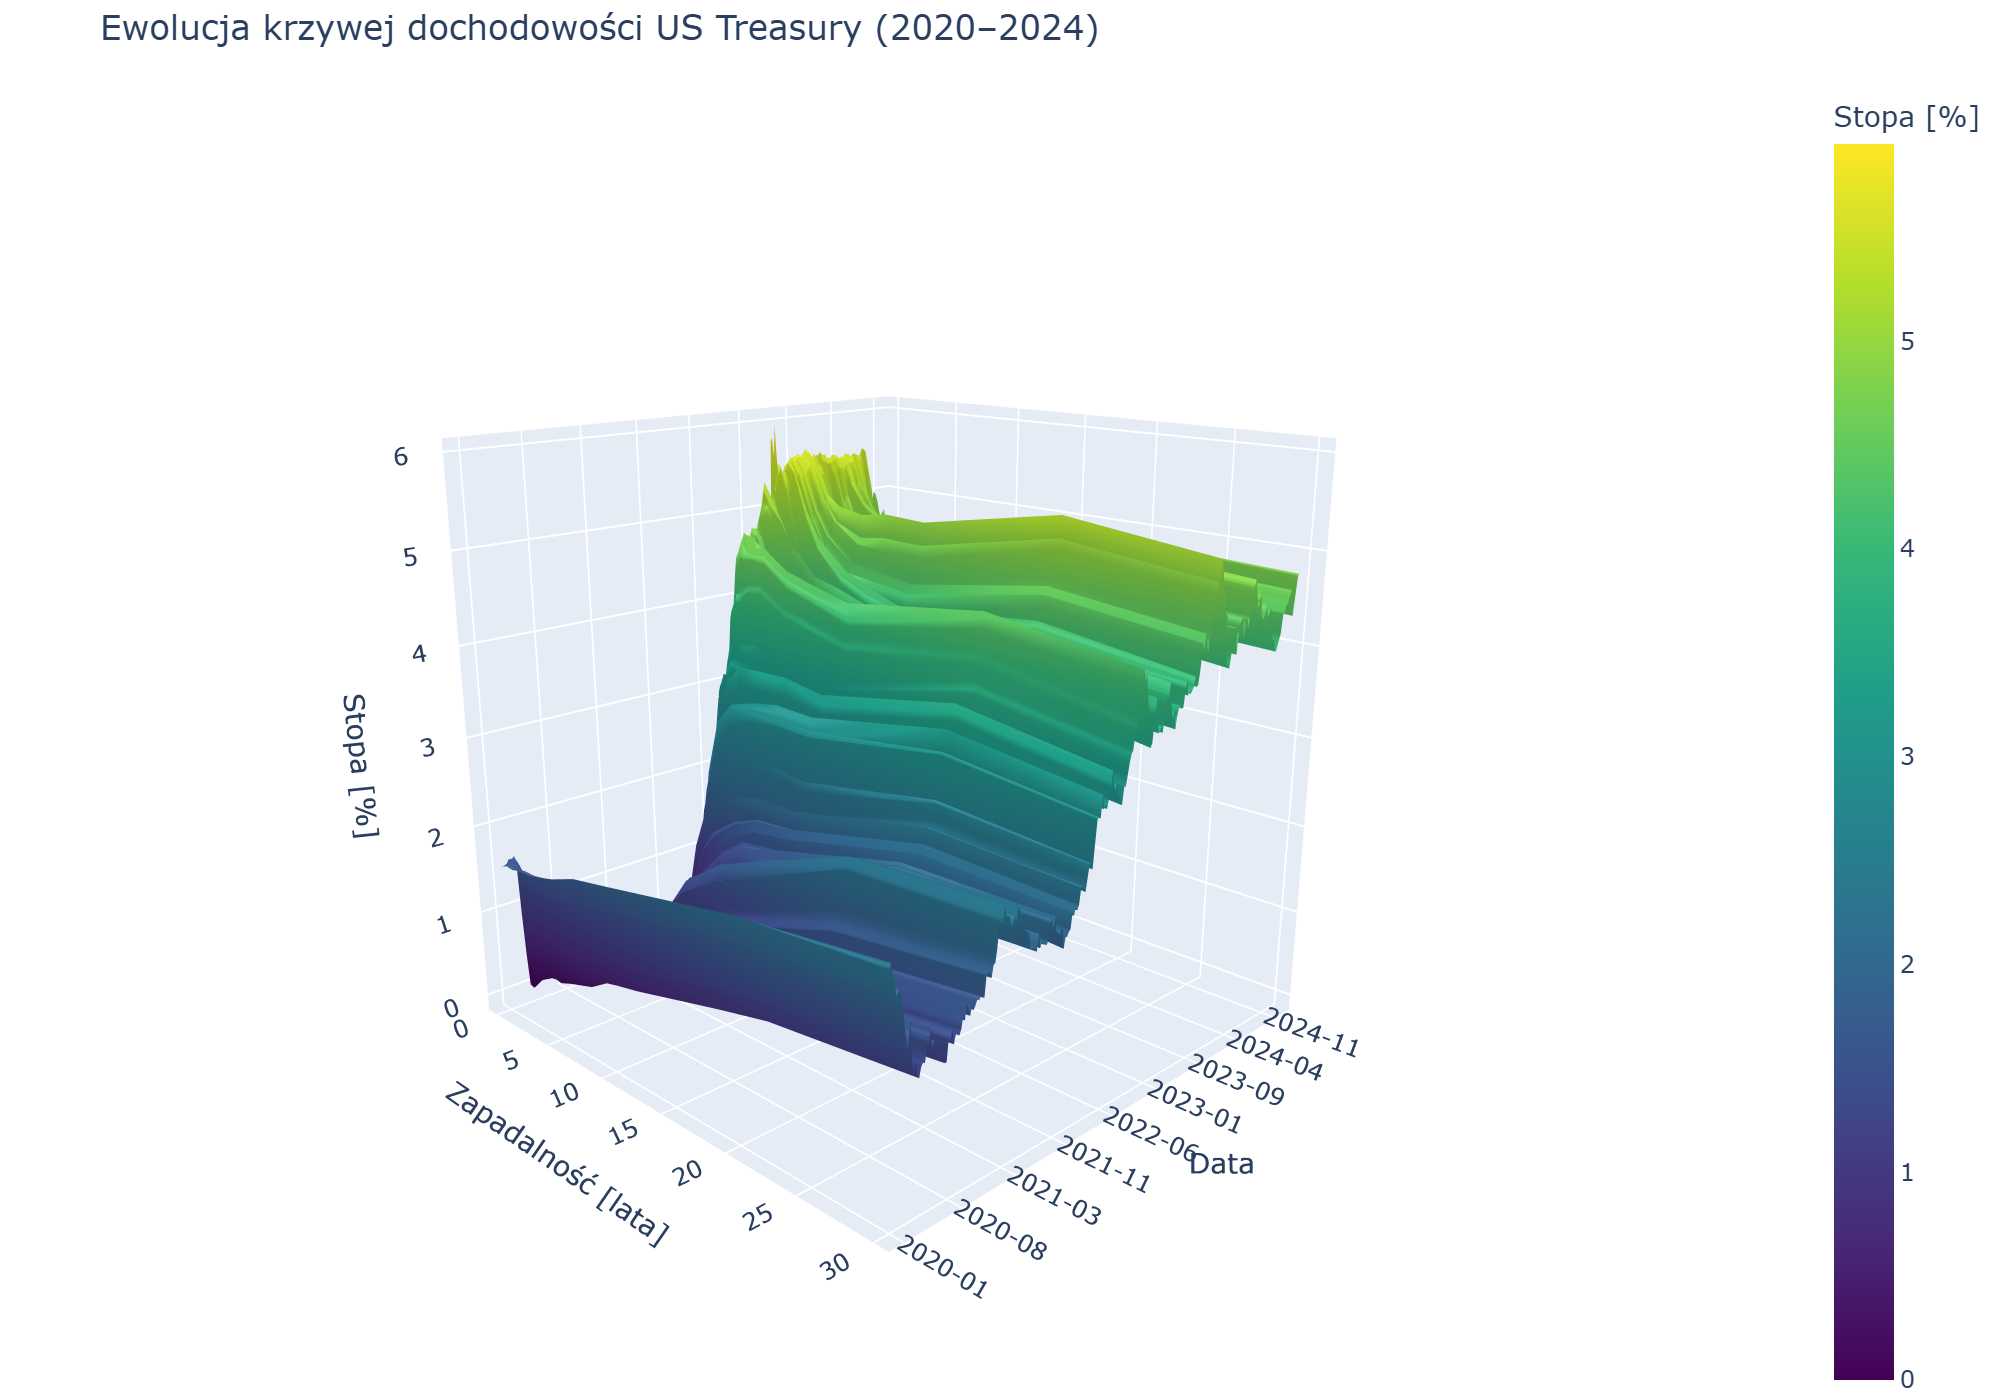
\includegraphics[width=\textwidth]{yield_curve_3d.png}
  \caption{Powierzchnia 3D ewolucji krzywej dochodowości US~Treasury
           (2020--2024). Osie: zapadalność $\times$ data $\times$ stopa.}
  \label{fig:yield-3d}
\end{figure}

% ══════════════════════════════════════════════════════════════════════════
\section{Kalibracja modelu}
\label{sec:calibration}

\subsection{Metodologia}

Parametry $a$ i~$\sigma$ estymowano z~historycznego szeregu krótkiej stopy
dwoma metodami:

\paragraph{OLS (Ordinary Least Squares).}
Regresja $\Delta r_i = \alpha + \beta\,r_i + \varepsilon_i$, skąd:
\begin{equation}
  a = -\frac{\beta}{\Delta t}, \qquad
  \sigma = \frac{\text{std}(\varepsilon)}{\sqrt{\Delta t}}.
\end{equation}

\paragraph{MLE (Maximum Likelihood Estimation).}
Estymacja pełnego modelu OU z~rozkładem warunkowym:
\begin{equation}
  r_{t+\Delta t} \mid r_t \sim \mathcal{N}\!\Bigl(
    r_t\,e^{-a\Delta t} + b\,(1-e^{-a\Delta t}),\;
    \frac{\sigma^2}{2a}(1-e^{-2a\Delta t})
  \Bigr).
\end{equation}

\subsection{Wyniki kalibracji}

\begin{table}[H]
  \centering
  \caption{Wyniki kalibracji na~całym okresie 2020--2024.}
  \label{tab:calibration}
  \begin{tabular}{@{}lccc@{}}
    \toprule
    \textbf{Metoda} & $a$ & $\sigma$ & $b$ (średnia długoterm.) \\
    \midrule
    OLS & 0,0010 & 0,0059 & $-1,3569$ \\
    MLE & 0,0010 & 0,0059 & $-1,6350$ \\
    \bottomrule
  \end{tabular}
\end{table}

\paragraph{Interpretacja.}
Bardzo niskie $a \approx 0{,}001$ (praktycznie brak mean-reversion)
wynika z~tego, że w~analizowanym okresie stopy wykazywały silny
\textbf{trend} (z~0\% do~5,5\%), a~nie stacjonarne wahania wokół średniej.
Jest~to ważna obserwacja: model OU ma trudności z~uchwyceniem strukturalnych
zmian reżimu polityki monetarnej.

\subsection{Krocząca kalibracja}

Aby~uchwycić zmienność parametrów w~czasie, przeprowadzono kroczącą
kalibrację w~oknie 60~dni roboczych (Rys.~\ref{fig:calibration}).

\begin{figure}[H]
  \centering
  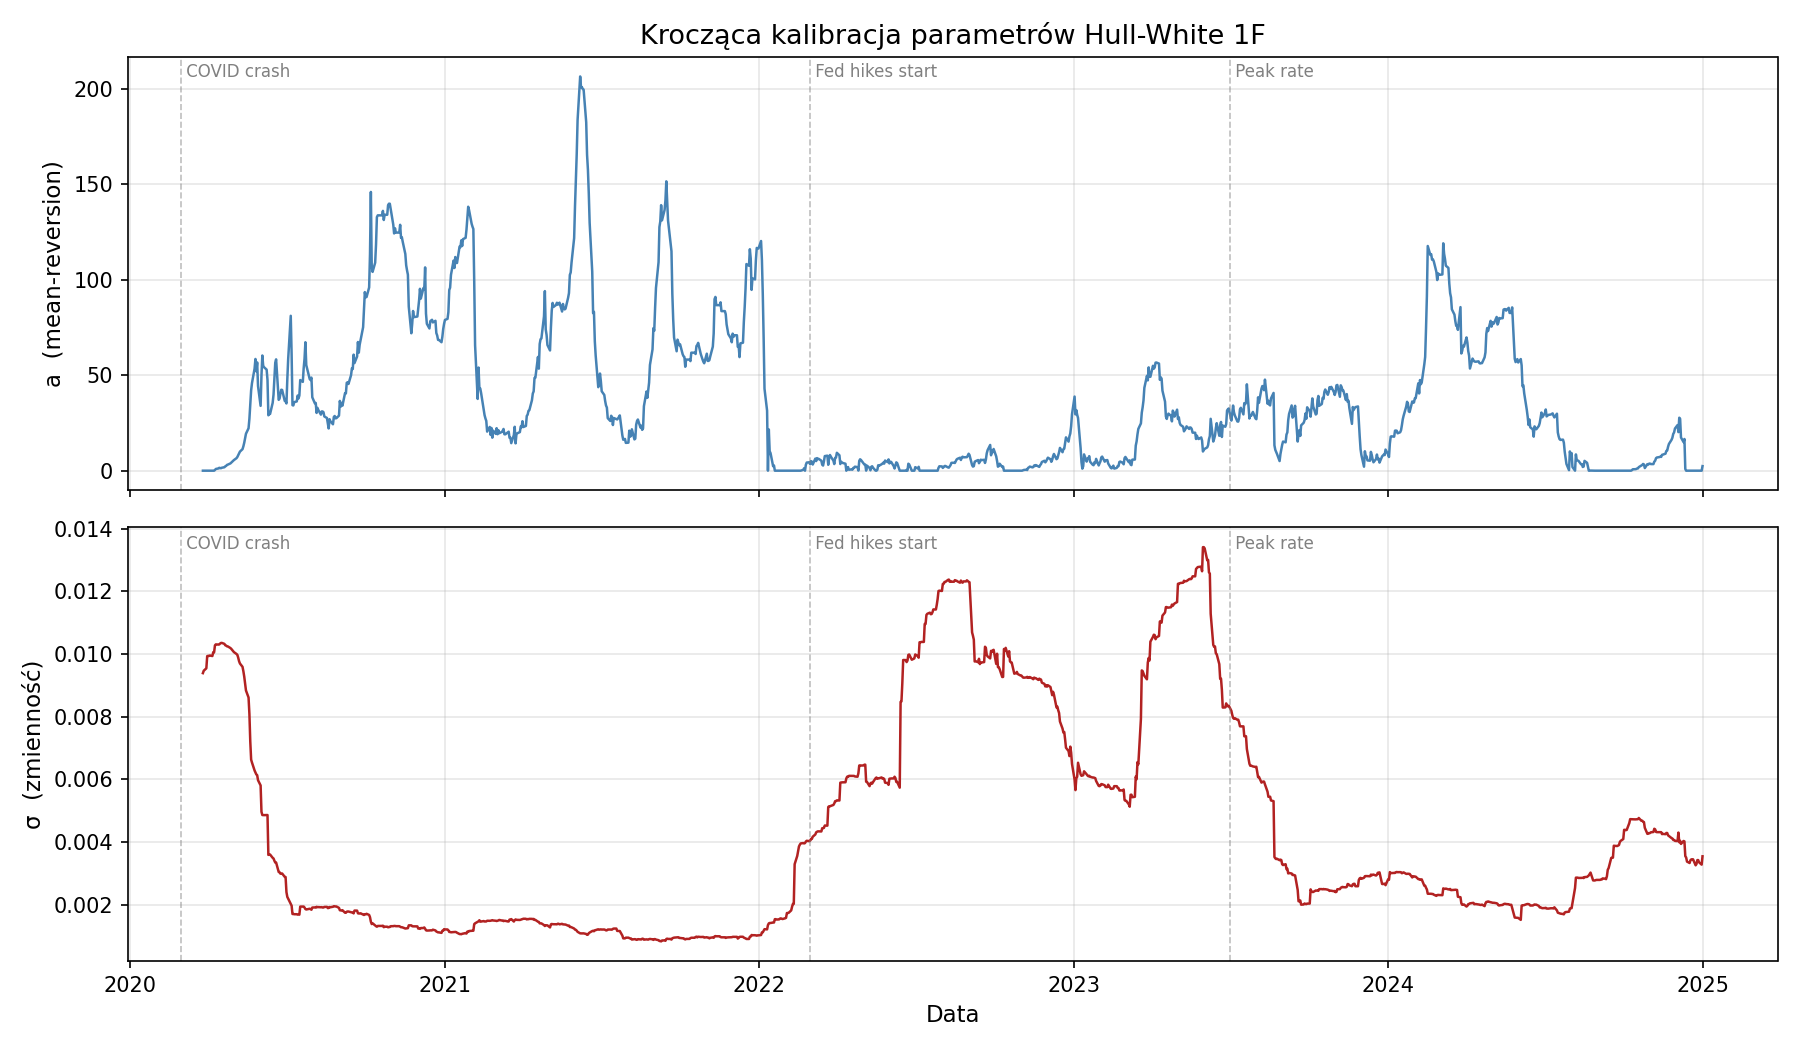
\includegraphics[width=\textwidth]{calibration_params.png}
  \caption{Krocząca kalibracja parametrów $a(t)$ i~$\sigma(t)$ modelu
           Hull-White~1F. Zaznaczono kluczowe wydarzenia makroekonomiczne:
           COVID crash (03/2020), początek podwyżek Fed (03/2022),
           szczyt stóp (07/2023).}
  \label{fig:calibration}
\end{figure}

Na wykresie widoczne są:
\begin{itemize}
  \item \textbf{Skoki $\sigma$} w~okresach turbulencji (COVID, początek
        cyklu podwyżek) -- rynek obligacji wykazywał podwyższoną zmienność;
  \item \textbf{Niestabilność $a$} -- parametr mean-reversion oscyluje,
        co~potwierdza, że w~krótkich oknach zachowanie stóp bywa
        niejednorodne.
\end{itemize}

% ══════════════════════════════════════════════════════════════════════════
\section{Wycena opcji na ZCB}
\label{sec:pricing}

\subsection{Parametry opcji}

Wyceniono europejską opcję call na~ZCB z~następującymi parametrami
(na~bazie krzywej z~31.12.2024):

\begin{table}[H]
  \centering
  \caption{Parametry wycenianej opcji.}
  \label{tab:option-params}
  \begin{tabular}{@{}ll@{}}
    \toprule
    \textbf{Parametr} & \textbf{Wartość} \\
    \midrule
    Czas wygaśnięcia opcji ($T$) & 1 rok \\
    Zapadalność obligacji ($S$)  & 5 lat \\
    Strike ($K$, ATM-forward)    & 0,8374 \\
    Bieżąca stopa $r(0)$        & 4,39\% \\
    $P^M(0,T)$                   & 0,9593 \\
    $P^M(0,S)$                   & 0,8033 \\
    \bottomrule
  \end{tabular}
\end{table}

Strike ustalono jako ATM-forward:
$K = P^M(0,S)\,/\,P^M(0,T) \approx 0{,}8374$.

\subsection{Wyniki wyceny}

\begin{table}[H]
  \centering
  \caption{Cena opcji call i~put na~ZCB.}
  \label{tab:prices}
  \begin{tabular}{@{}lc@{}}
    \toprule
    \textbf{Opcja}  & \textbf{Cena} \\
    \midrule
    Call (analityczna HW) & 0,007628 \\
    Put (analityczna HW)  & 0,007585 \\
    Call (Monte Carlo)    & 0,007578 $\pm$ 0,000113 \\
    \bottomrule
  \end{tabular}
\end{table}

Parytet put-call jest spełniony:
$C - P = 0{,}000043 \approx P(0,S) - K \cdot P(0,T) = 0{,}000042$.

% ══════════════════════════════════════════════════════════════════════════
\section{Symulacja Monte Carlo}
\label{sec:mc}

\subsection{Schemat Eulera-Maruyamy}

Ścieżki krótkiej stopy generowano schematem Eulera-Maruyamy:

\begin{equation}
  r_{i+1} = r_i + \bigl[\theta(t_i) - a\,r_i\bigr]\Delta t
           + \sigma\sqrt{\Delta t}\,Z_i,
  \qquad Z_i \sim \mathcal{N}(0,1).
\end{equation}

Parametry symulacji: 10\,000~ścieżek, 252~kroki (dzienne), horyzont 1~rok.

\subsection{Weryfikacja ceny analitycznej}

Rysunek~\ref{fig:mc-dist} zestawia rozkład zdyskontowanych payoffów MC
z~ceną analityczną.

\begin{figure}[H]
  \centering
  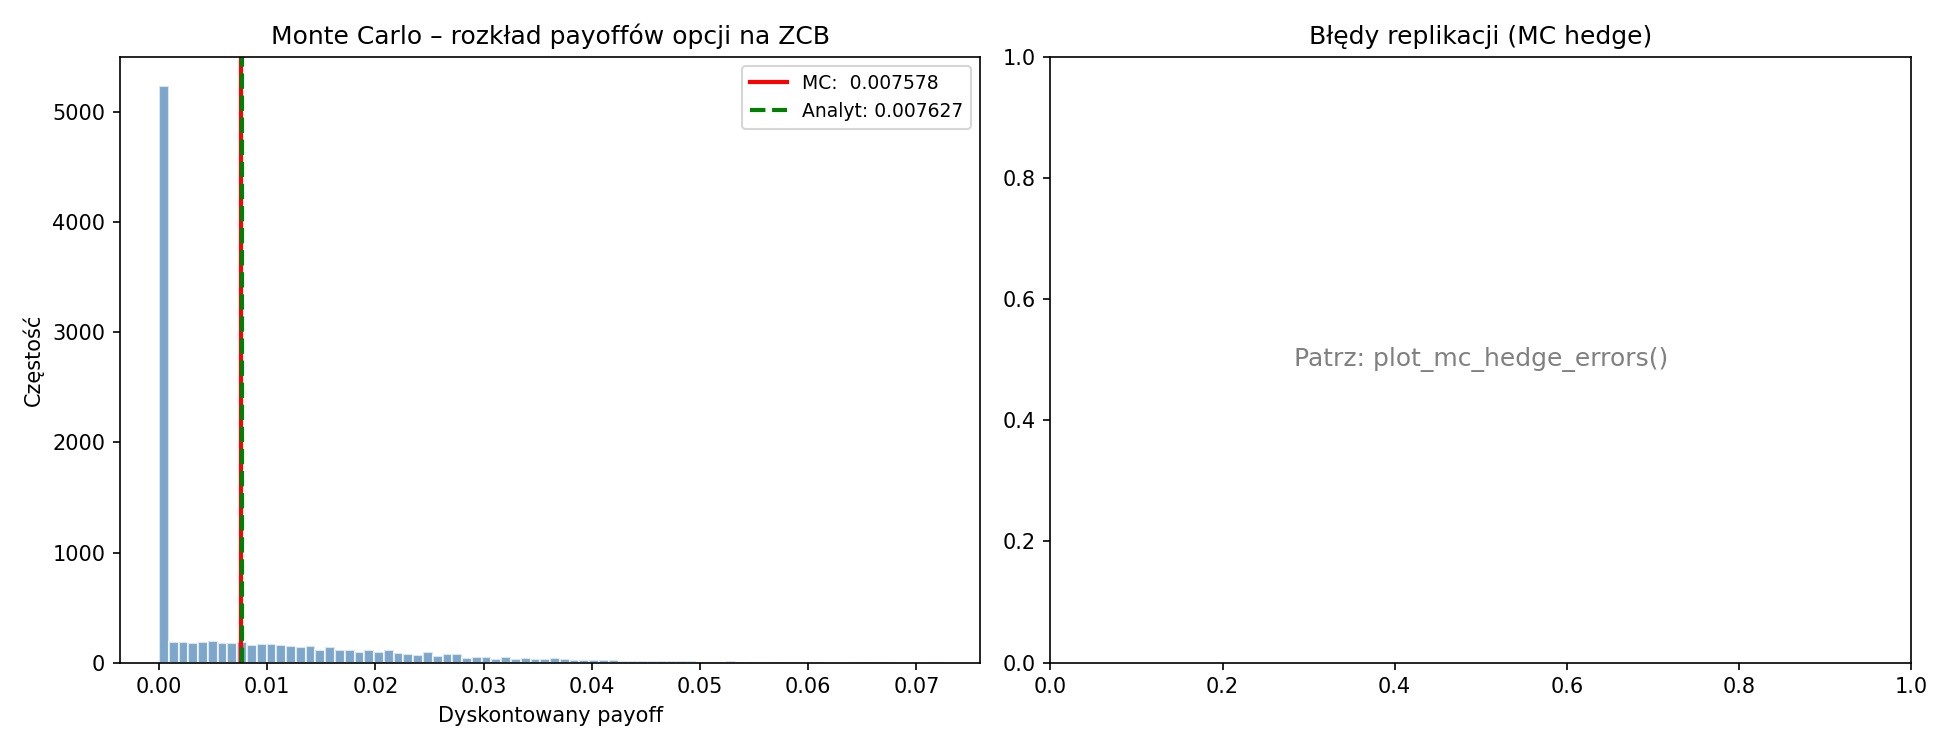
\includegraphics[width=\textwidth]{mc_distribution.png}
  \caption{Monte Carlo: rozkład zdyskontowanych payoffów opcji call.
           Czerwona linia -- średnia MC ($0{,}007578$), zielona przerywana --
           cena analityczna ($0{,}007628$). Różnica: $0{,}000049$.}
  \label{fig:mc-dist}
\end{figure}

Zgodność MC z~wynikiem analitycznym (różnica $< 1$~błędu standardowego)
potwierdza poprawność implementacji zarówno formuły Jamshidiana, jak
i~schematu symulacji.

% ══════════════════════════════════════════════════════════════════════════
\section{Delta-Hedging}
\label{sec:hedging}

\subsection{Strategia zabezpieczająca}

Strategia delta-hedgingu polega na:
\begin{enumerate}
  \item Sprzedaży opcji call (otrzymanie premii $C_0$);
  \item Zakupie $\Delta_0 = \Phi(h_0)$ jednostek obligacji $P(0,S)$;
  \item Okresowym rebalansowaniu pozycji (tygodniowo lub dziennie);
  \item Na~koniec: porównaniu wartości portfela z~payoffem opcji.
\end{enumerate}

Błąd replikacji (\emph{hedge error}):
\begin{equation}
  \varepsilon_{\text{hedge}} = V_T^{\text{portfolio}} - \max\bigl(P(T,S) - K,\;0\bigr).
\end{equation}

\subsection{Backtest na ścieżkach Monte Carlo}

Przeprowadzono backtest na~5000~ścieżkach MC z~tygodniowym rebalansem
(52~kroki).

\begin{table}[H]
  \centering
  \caption{Wyniki delta-hedgingu MC.}
  \label{tab:hedge-mc}
  \begin{tabular}{@{}lc@{}}
    \toprule
    \textbf{Metryka} & \textbf{Wartość} \\
    \midrule
    Premia opcji $C_0$         & 0,007627 \\
    MAE (błąd replikacji)      & 0,001464 \\
    $\sigma$ (błąd replikacji) & 0,001809 \\
    \bottomrule
  \end{tabular}
\end{table}

\begin{figure}[H]
  \centering
  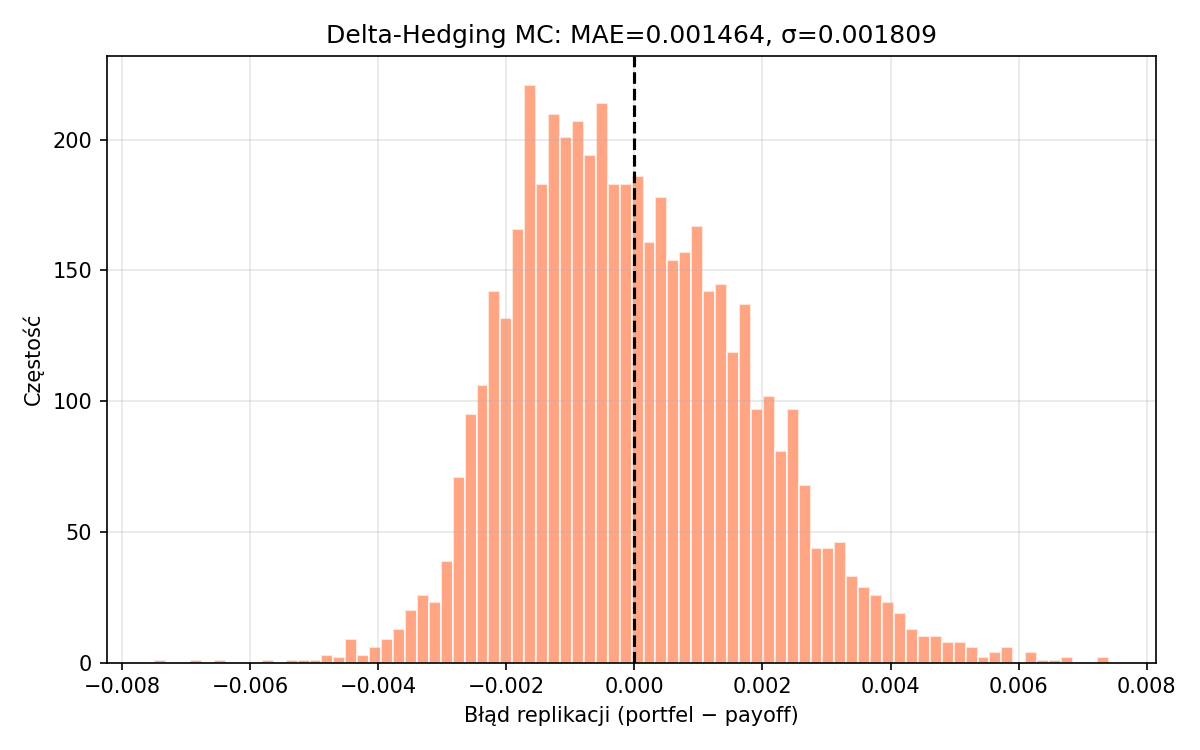
\includegraphics[width=0.85\textwidth]{mc_hedge_errors.png}
  \caption{Histogram błędów replikacji z~MC delta-hedgingu.
           Rozkład jest skupiony wokół zera -- hedging działa poprawnie
           w~świecie modelu.}
  \label{fig:mc-hedge}
\end{figure}

\subsection{Backtest na danych historycznych}

Kluczowy test: czy model działa na \textbf{rzeczywistych} danych?
Przeprowadzono backtest z~4~różnymi datami startu, każdorazowo
z~opcją 1-roczną na~ZCB 5-letni.

\begin{table}[H]
  \centering
  \caption{Wyniki historycznego delta-hedgingu.}
  \label{tab:hedge-hist}
  \begin{tabular}{@{}lccc@{}}
    \toprule
    \textbf{Start} & \textbf{Premia $C_0$} & \textbf{Payoff} &
      \textbf{Hedge error} \\
    \midrule
    2020-06 & 0,1486 & 0,1404 & $+0{,}0008$ \\
    2021-06 & 0,1232 & 0,0587 & $-0{,}0010$ \\
    2022-01 & 0,0997 & 0,0158 & $-0{,}0211$ \\
    2023-01 & 0,0236 & 0,0161 & $-0{,}0151$ \\
    \bottomrule
  \end{tabular}
\end{table}

\begin{figure}[H]
  \centering
  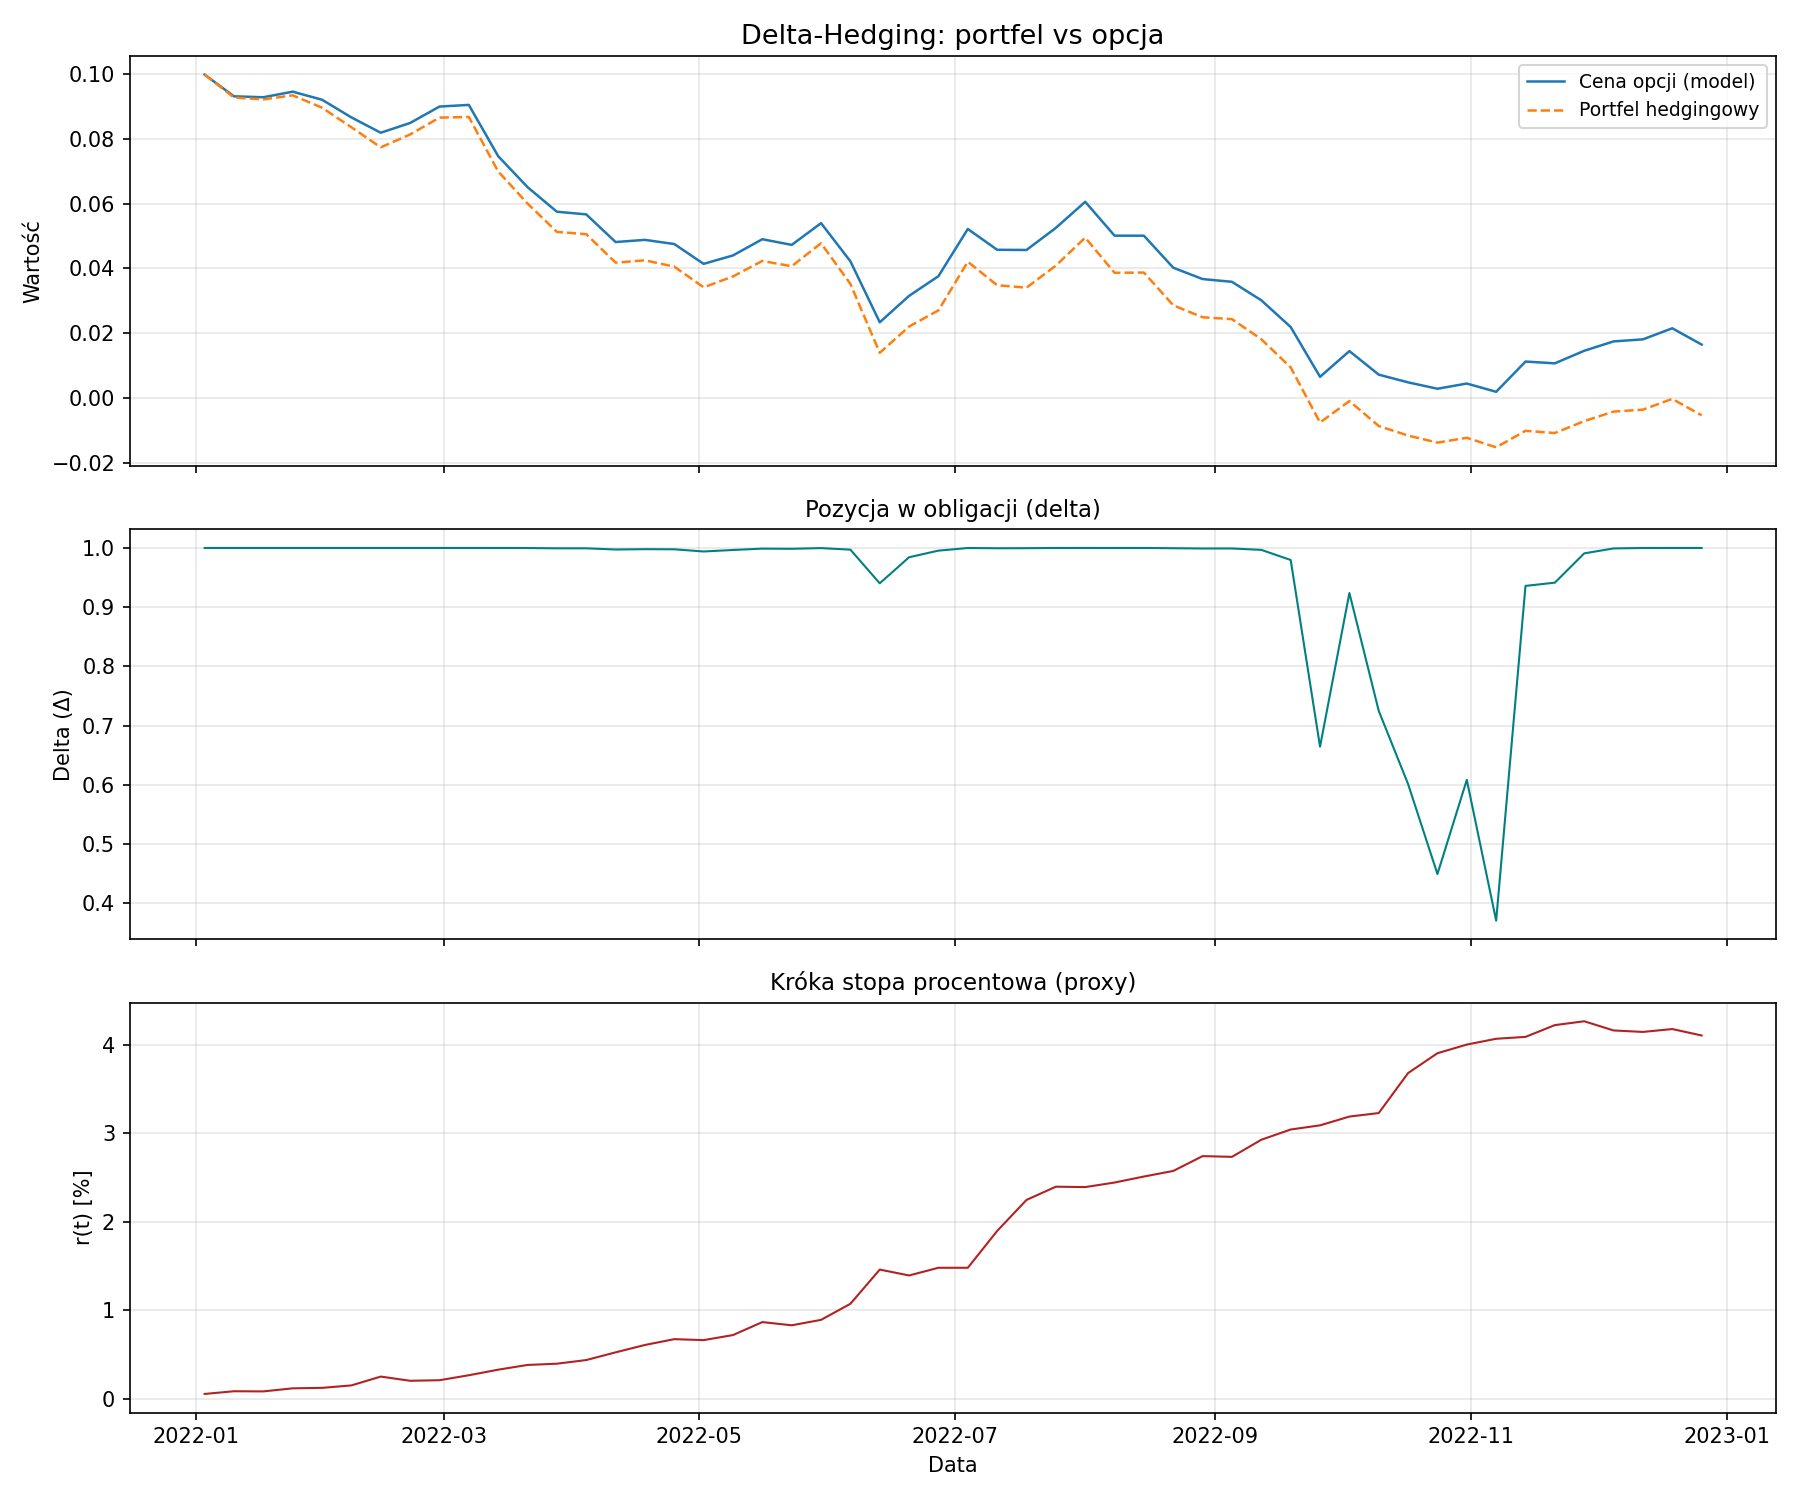
\includegraphics[width=\textwidth]{hedging_pnl.png}
  \caption{Historyczny delta-hedging -- okres startowy 01/2022.
           Panel~górny: wartość portfela hedgingowego vs cena opcji.
           Panel~środkowy: pozycja delta. Panel~dolny: proxy krótkiej stopy.}
  \label{fig:hedge-hist}
\end{figure}

\paragraph{Interpretacja wyników.}
\begin{itemize}
  \item Okresy \textbf{2020--2021} (stabilne/malejące stopy): hedging
        działa bardzo dobrze, błąd $< 0{,}001$.
  \item Okres \textbf{2022} (agresywne podwyżki): błąd rośnie do~$0{,}021$
        -- model nie przewiduje tak gwałtownych zmian reżimu.
  \item Okres \textbf{2023} (stabilizacja na~szczycie): błąd $0{,}015$ --
        hedging częściowo się odbudowuje, ale~stopy utrzymują się na~poziomie
        nieprzewidzianym przez parametry skalibrowane wcześniej.
\end{itemize}

Jest~to kluczowy wniosek projektu: \textbf{delta-hedging oparty na~modelu
HW~1F jest skuteczny w~normalnych warunkach, ale~jego jakość pogarsza się
w~okresach strukturalnych zmian polityki monetarnej}, gdy założenie
o~stacjonarności procesu stopy jest naruszone.

% ══════════════════════════════════════════════════════════════════════════
\section{Porównanie Hull-White vs Vasicek}
\label{sec:comparison}

\begin{figure}[H]
  \centering
  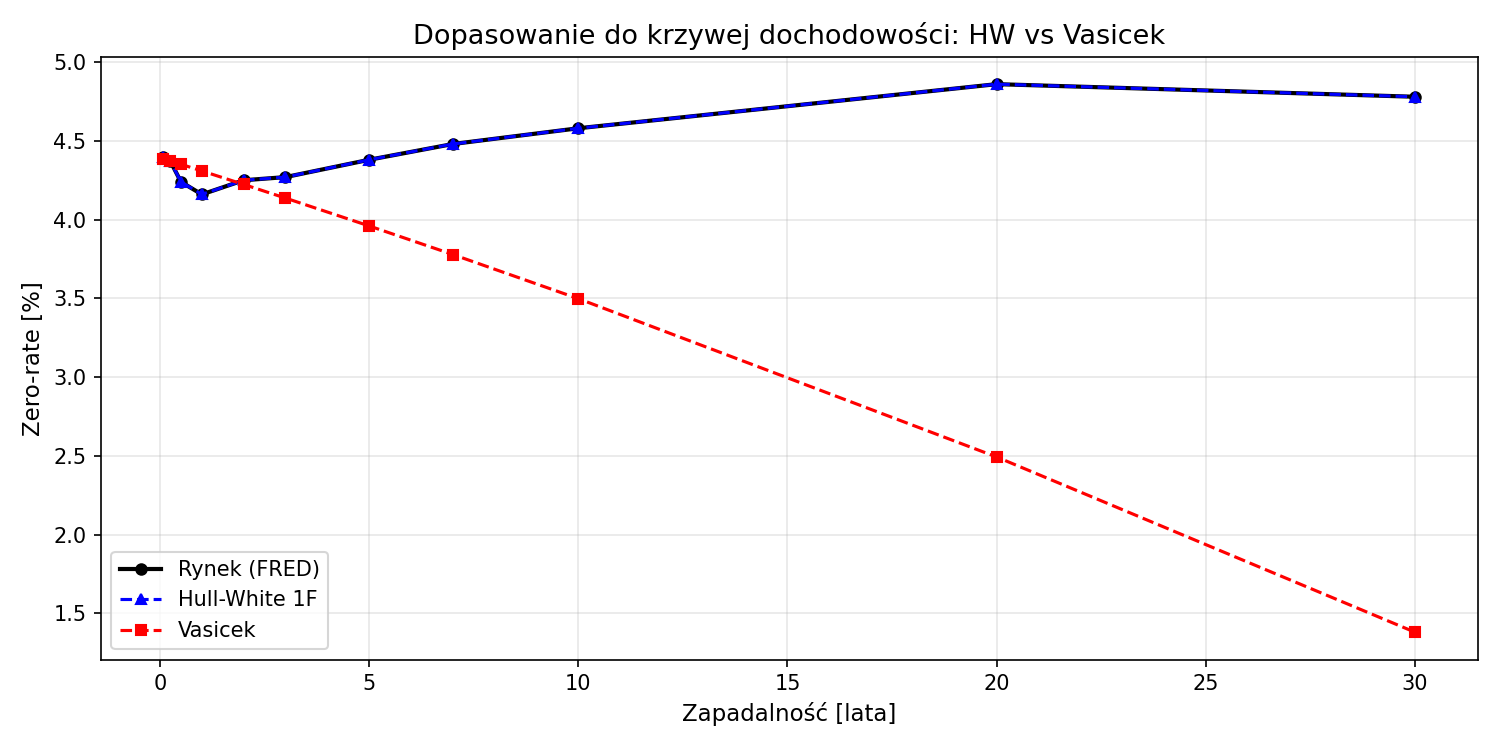
\includegraphics[width=\textwidth]{hw_vs_vasicek.png}
  \caption{Dopasowanie do krzywej dochodowości: Hull-White~1F vs Vasicek.
           HW idealnie odtwarza krzywą rynkową (RMSE~$=0$~bps), Vasicek
           wykazuje systematyczne odchylenie ($131{,}6$~bps).}
  \label{fig:hw-vs-vasicek}
\end{figure}

\begin{table}[H]
  \centering
  \caption{Porównanie modeli.}
  \label{tab:comparison}
  \begin{tabular}{@{}lcc@{}}
    \toprule
    \textbf{Metryka} & \textbf{Hull-White 1F} & \textbf{Vasicek} \\
    \midrule
    RMSE krzywej [bps]    & 0,0    & 131,6   \\
    Cena call              & 0,0076 & 0,0201  \\
    Dopasowanie do $P^M(0,T)$ & dokładne & przybliżone \\
    Funkcja $\theta(t)$   & zmienna & stała ($=ab$) \\
    \bottomrule
  \end{tabular}
\end{table}

Przewaga Hull-White wynika z~deterministycznej funkcji $\theta(t)$,
która zapewnia \textbf{brak arbitrażu} względem obserwowanej krzywej
dochodowości. Vasicek z~ustalonym $b$ generuje krzywą modelową
odchyloną o~ponad 130~bps od~rynkowej, co~prowadzi do systematycznego
błędu wyceny instrumentów pochodnych.

% ══════════════════════════════════════════════════════════════════════════
\section{Architektura implementacji}
\label{sec:architecture}

Projekt zaimplementowano w~Pythonie w~architekturze modułowej:

\begin{table}[H]
  \centering
  \caption{Struktura modułów projektu.}
  \label{tab:modules}
  \begin{tabular}{@{}lp{8cm}@{}}
    \toprule
    \textbf{Moduł} & \textbf{Odpowiedzialność} \\
    \midrule
    \texttt{data/}         & Pobieranie danych z~FRED, konstrukcja
                             krzywej (splajn kubiczny) \\
    \texttt{models/}       & Hull-White~1F (analityka, ZCB, opcje,
                             delta) oraz Vasicek \\
    \texttt{calibration/}  & Kalibracja OLS, MLE, krocząca \\
    \texttt{simulation/}   & Euler-Maruyama MC, wycena MC \\
    \texttt{hedging/}      & Delta-hedging: backtest MC
                             i~historyczny \\
    \texttt{visualization/}& Wykresy: 3D krzywa, kalibracja,
                             hedging, porównania \\
    \texttt{main.py}       & Orkiestrator 8-krokowego pipeline'u \\
    \bottomrule
  \end{tabular}
\end{table}

Kluczowe biblioteki: NumPy, SciPy (optymalizacja, interpolacja),
Pandas (szeregi czasowe), Matplotlib/Plotly (wizualizacja),
fredapi (dane FRED).

% ══════════════════════════════════════════════════════════════════════════
\section{Wnioski}
\label{sec:conclusions}

\begin{enumerate}
  \item \textbf{Model Hull-White~1F idealnie odtwarza krzywą dochodowości}
        dzięki funkcji $\theta(t)$, w~przeciwieństwie do~modelu Vasicka
        (RMSE: 0~vs~132~bps).

  \item \textbf{Ceny analityczne i~MC są spójne} -- różnica $<0{,}005\%$
        wartości opcji, co~potwierdza poprawność implementacji.

  \item \textbf{Delta-hedging jest skuteczny w~normalnych warunkach}
        (błąd $\sim 0{,}1\%$ premii), ale~pogarsza się w~okresach
        strukturalnych szoków stóp (2022: błąd $\sim 2\%$~nominału).

  \item \textbf{Kalibracja historyczna ma ograniczenia}: w~okresie silnego
        trendu stóp (2020--2023) parametr mean-reversion $a$ jest bliski
        zeru, co~oznacza, że~model OU nie~jest w~stanie uchwycić zmiany
        reżimu polityki monetarnej.

  \item \textbf{Potencjalne rozszerzenia}:
        \begin{itemize}
          \item model dwuczynnikowy (HW~2F lub G2++) dla~lepszego
                dopasowania do~zmienności;
          \item kalibracja do~cen rynkowych swaptionów/capów zamiast
                estymacji historycznej;
          \item parametry zależne od~reżimu (\emph{regime-switching}).
        \end{itemize}
\end{enumerate}

% ══════════════════════════════════════════════════════════════════════════
\section*{Bibliografia}

\begin{enumerate}
  \item Hull, J.\,C., White, A. (1990). \textit{Pricing Interest-Rate
        Derivative Securities}. The Review of Financial Studies, 3(4),
        573--592.

  \item Brigo, D., Mercurio, F. (2006). \textit{Interest Rate Models --
        Theory and Practice}. Springer, 2nd edition.

  \item Vasicek, O. (1977). \textit{An Equilibrium Characterization of the
        Term Structure}. Journal of Financial Economics, 5(2), 177--188.

  \item Jamshidian, F. (1989). \textit{An Exact Bond Option Formula}.
        The Journal of Finance, 44(1), 205--209.

  \item Federal Reserve Bank of St.~Louis (2024). \textit{FRED Economic
        Data}. \url{https://fred.stlouisfed.org}.
\end{enumerate}

\end{document}
